\documentclass[border=2pt, 10pt]{standalone}

\usepackage[dvipsnames]{xcolor}
    \definecolor{GDLcolor}{HTML}{A6A6A6}
    \definecolor{ELcolor}{HTML}{E8E490}
\usepackage{tikz}
    \usetikzlibrary{math, calc}
\usepackage{siunitx}
\sisetup{%
    mode=math,
    per-mode=power,
}

\begin{document}
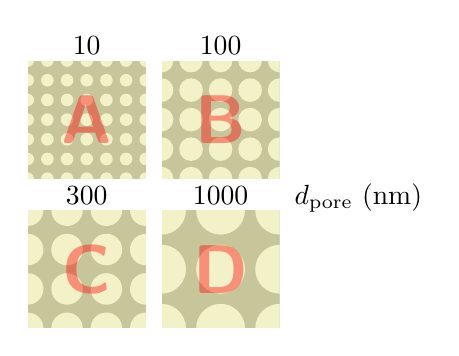
\begin{tikzpicture}
    \tikzset{%
        pics/dpore/.style args={#1/#2/#3/#4}{code={%
                        \tikzmath{%
                            \dpore=#1;
                            \deltafig=1.5;
                            \numpore=#2;
                            \deltawall=(\deltafig-\numpore*\dpore)/\numpore;
                        };

                        \begin{scope}
                            \clip (0, 0) rectangle ++(\deltafig, \deltafig);
                            GDL
                            \fill [GDLcolor] (0, 0) rectangle ++(\deltafig, \deltafig);
                            % pore
                            \foreach \i in {0, ..., \numpore} {%
                                    \foreach \j in {0, ..., \numpore} {%
                                            \fill [white] ({\i*(\dpore+\deltawall)}, {\j*(\dpore+\deltawall)}) circle (\dpore);
                                        }
                                };
                            % EL
                            \fill [ELcolor, opacity=0.5] (0, 0) rectangle ++(\deltafig, \deltafig);
                        \end{scope}

                        \node at (\deltafig/2, \deltafig-0.05) [above] {\ensuremath{#3}};
                        \node at (\deltafig/2, \deltafig/2) [opacity=0.4] {\sffamily\bfseries\color{red}\fontsize{30pt}{30pt}\selectfont #4};
                    }
            }
    }

    % dpore/numpore/dpore text/A
    \pic at (0, 0) {dpore=0.08/6/10/A};
    \pic at (1.7, 0) {dpore=0.15/4/100/B};
    \pic at (0, -1.9) {dpore=0.2/3/300/C};
    \pic at (1.7, -1.9) {dpore=0.31/2/1000/D};
    \node at (4.2, -0.25) {$ d_{\mathrm{pore}}~(\unit{\nano\meter}) $};

\end{tikzpicture}
\end{document}